\documentclass[a4paper, 12pt, oneside]{scrartcl}
\usepackage[utf8]{inputenc}

\input{../../header.tex}

\title{Coursera ML Notes\\\large Stanford: Andrew Ng's ``Machine Learning''}
\author{Lectures by Andrew Ng\\Notes by Matthew Low \texttt{mattchrlw}}
\date{\today}

\begin{document}

\maketitle

\tableofcontents

\section{Week 1}

\subsection{Introduction}
Pretty simple stuff. House price example, news classification example etc. etc.

\subsection{Model and cost function}
Let $x^{(i)}$ denote the ``input'' variables/features, and $y^{(i)}$ denote the ``output'' or target variable we wish to predict. A pair $(x^{(i)}, y^{(i)})$ is called a \textbf{training example}, and the dataset that we'll be using to learn:
\[(x^{(i)}, y^{(i)}), \quad i = 1,\ldots, m,\]
is called a \textbf{training set}. Superscript denotes an index into the training set, which isn't too bad notation when you start looking at gradient descent etc. For the purposes of this introductory course, we use $X$ to denote the space of input values and $Y$ to denote the space of output values, and $X = Y = \mathbb R$.

In supervised learning, the goal is given a training set to learn a function $h: X \to Y$ such that $h(x)$ is a good predictor for $y$. $h$ is called a \textbf{hypothesis} for historical reasons. Discrete $\implies$ classification, continuous $\implies$ regression (but it can be more complicated than that.

To measure the accuracy of our hypothesis function (in linear regression), we can use a \textbf{cost function}. In the context of linear regression, this cost function is least squares.
\[J(\theta_0, \theta_1) = \frac{1}{2m} \sum_{i=1}^m (h_\theta(x_i) - y_i)^2 \quad \equiv \quad \frac12 \|Hx - y\|^2,\]
where $H$ is some matrix but that isn't important for this since we are using \textit{Ng-otation} and I just wanted to show it's OLS. The function is called the ``squared error function'', ``mean squared error'' or MSE. The mean is halved as a convenience for gradient descent (because the squared carries over to the fraction, useful for the normal equation). Since this function represents the \textit{cost}, we wish to minimise it.

\begin{figure}[H]
\centering
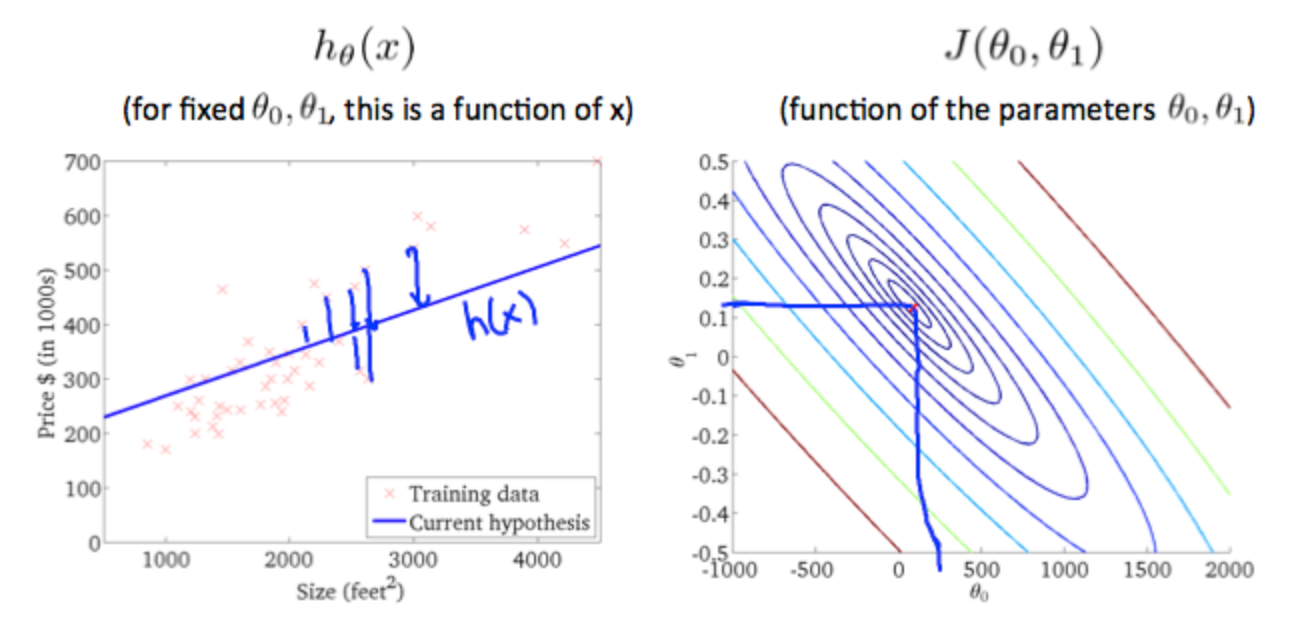
\includegraphics[width=0.6\textwidth]{figures/contour.png}
\end{figure}

\subsection{Parameter learning}

We want to estimate the parameters in the hypothesis function, which is where \textbf{gradient descent} comes in. Graphing our hypothesis function as a function of the parameter estimates gives a surface. Gradient descent uses the fact that the gradient is the direction towards the minimum (very roughly speaking) to perform an iterative movement towards the minimum. I would write more detail about gradient descent but I'm literally doing a summer project on optimisation so I don't think there's much point, refer to my optimisation notes for more details. This algorithm gives an iterate
\[\theta_j := \theta_j - \alpha \frac{\partial}{\partial \theta_j} J(\theta_0, \theta_1),\]
where $j=0,1$ represents the feature index number.
\begin{center}
    \textit{Update the parameters simultaneously, or else gradient descent won't work!}
\end{center}
(Note: this fact would be obvious if we employed the gradient operator $\nabla J(\theta_0, \theta_1)$ instead of Ng's notation, but I digress.)

When specially applied to linear regression, we can obtain a new form of gradient descent. Replacing the cost function and hypothesis function, we obtain the following iterate:
\begin{align*}
    \theta_0 &:= \theta_0 - \alpha \frac1m \sum_{i=1}^m (h_\theta(x_i) - y_i) \\
    \theta_1 &:= \theta_1 - \alpha \frac1m \sum_{i=1}^m ((h_\theta(x_i) - y_i)x_i)
\end{align*}
These can both be verified with some calculus.

\section{Week 2}

\subsection{Multivariate linear regression}

Linear regression with multiple variables is also known as \textbf{multivariate linear regression}. In the more general case, we can have the following:

\begin{center}
    \begin{tabular}{cl}
     $x_j^{(i)}$ & value of feature $j$ in the $i$th training example \\
     $x^{(i)}$ & the input of the $i$th training example \\
     $m$ & the number of training examples \\
     $n$ & the number of features
    \end{tabular}
\end{center}
The multivariate form of this is
\[h_\theta(x) = \theta_0 + \theta_1 x_1 + \theta_2 x_2 + \ldots + \theta_n x_n \quad \equiv \quad h_\theta(x) = \theta^\top x\]
where $\theta = \begin{pmatrix} \theta_0 & \theta_1 & \ldots & \theta_n \end{pmatrix}$ and $x = \begin{pmatrix} x_0 & x_1 & \ldots & x_n \end{pmatrix}^\top$.

For gradient descent in the multivariate case using Ng's notation we have the following iterate:
\[\theta_j := \theta_j - \alpha \frac1m \sum_{i=1}^m (h_\theta(x^{(i)} - y^{(i)}) \cdot x_j^{(i)}, \quad \forall j \in \{0, \ldots, n\}.\]

We introduce a practical trick for gradient descent called \textbf{feature scaling}. The idea is to ensure that features are on a similar scale, making gradient descent faster. We get every feature into \textit{approximately} a $-1 \leq x_i \leq 1$ range. You can also perform \textbf{mean normalisation}, where we replace $x_i$ with $x_i - \mu_i$ to make features have approximately zero mean, making sure not to apply to $x_0 = 1$ or anything like that. You can also divide by the standard deviation $s_i$ instead of the range.

For gradient descent, we can also use something called the \textbf{automatic convergence test}. Declare convergence if $J(\theta)$ decreases by less than $\varepsilon$ in one iteration, where $\varepsilon$ is some small value. (It's difficult to choose this threshold value). If $\alpha$ is too small, we have a slow convergence rate, but if $\alpha$ is too large, we may not decrease on every iteration and thus may not converge.

We may also have a situation where we have polynomial regression. We can change the behaviour or curve of our hypothesis function by making it a quadratic, cubic or square root function (or any other form). For example, if our hypothesis function is $h_\theta(x) = \theta_0 + \theta_1 x$, we can create additional features based on $x_1$ to get a quadratic with $\theta_2 x_1^2$ or even a cubic with both $\theta_2 x_1^2$ and $\theta_3 x_1^3$ added.

\subsection{Computing parameters analytically}

We have been using iterative algorithms so far such as gradient descent, but for some problems we can solve for $\theta$ analytically. The \textbf{normal equation} formula (the Moore-Penrose pseudoinverse times $y$ for the enlightened) is the solution to the problem
\[\theta = (X^\top X)^{-1} X^\top y.\]
There is no need to do feature scaling or any other bollocks with the normal equation. However, the normal equation has complexity $\mathcal O(n^3)$ and you may need to compute the inverse of $X^\top X$, so it can be really slow for large $n$.

\begin{center}
\begin{tabular}{l|l}
Gradient Descent & Normal Equation \\
\hline
Need to choose $\alpha$ & No need to choose $\alpha$ \\
Needs many iterations & No need to iterate \\
$\mathcal O(kn^2)$ & $\mathcal O(n^3)$ and inverse \\
Works well when $n$ is large & Slow if $n$ is large
\end{tabular}
\end{center}

But look at the normal equation; we have an inverse. Not every matrix has an inverse. Using \texttt{pinv} in MATLAB gets around this in some fancy ways, but we should still be alarmed if $X^\top X$ is noninvertible, as there may be:
\begin{itemize}
    \item Redundant features, where two features are very closely related (linearly dependent)
    \item Too many features ($m \leq n$). In this case, delete some features or use ``regularisation''.
\end{itemize}

\end{document}
